\chapter{Robust Latch Designs for Multiple Node Upsets} \label{ch1}

The focus of this chapter is on the design of soft error hardened latches. There has been extensive research in the field of hardening latches against single even upsets (SEU). The simplest design for safety critical applications is the triple modular redundancy (TMR) latch. This design consists of three standard latches connected to a 3-input majority voting circuit. While this design is tolerant against errors, it has the drawback of high area, delay and power consumption. For this reason there have been many other designs proposed that offer high SEU reliability with lower area, delay and power consumption. The first and most common cell is the DICE cell proposed in \cite{DICE}. The DICE cell consists of eight cross-coupled PMOS and NMOS transistors connected in series which forms four nodes. Due to the relatively high delay and power consumption of the DICE latch, there have been many other SEU tolerant latch designs proposed that provide reliability using blocking Muller C-elements \cite{Muller1956}, redundancy or delay in the feedback path \cite{HIPER, FERST, Hazucha, SEMULatch, Multivdd, BISER, NicoFeedback}.

The further reduction of the transistor feature size has increase the likelihood of a single event causing a transient pulse on multiple nodes simultaneously, commonly referred to as a single event multiple upset (SEMU). This trend necessitates the development of new latch designs that are tolerant to multiple node strikes to guarantee reliability in current and future technologies. As in the SEU case, the goal of these designs is to minimize the power, delay and area overheads. However, contrary to the SEU case, the latches are designed to tolerate two simultaneous errors, commonly referred to as a double node upset (DNU). Currently there are many existing latch designs that are tolerant to DNUs which are discussed in Section \ref{sec:DNUex}.   

Many modern circuit designs employ a technique commonly referred to as clock gating to further reduce power consumption. Clock gating consists of setting the clock to a stable value or ``gating" the clock. If clock gating is used with a latch, it may need to hold the current state for many clock cycles. In the presence of DNUs, this increases the likelihood of multiple errors occurring during the hold phase. In many existing DNU tolerant designs, a DNU puts the latch to a high impedance state in which the correct value could be lost if the latch experiences a second SEU or DNU before the transparent mode. Additionally, if the latch is gated for a sufficient number of cycles, the data held in the latch may degrade. For this reason, there is a need for new designs that are capable of holding the correct output value after a DNU for any number of clock cycles. In this chapter, we classify all DNU tolerant designs as either DNU robust or DNU non-robust. A DNU robust design is defined as being capable of resisting further errors and by not allowing any high impedance states after a DNU occurs. A DNU non-robust design is a latch that does not meet the all of stated criteria. In this chapter, a novel latch design referred to as the HRDNUT (Highly Robust Double Node Upset Tolerant) is proposed.

\section{Background on Existing DNU Tolerant Latches} \label{sec:DNUex}

Currently, there are a few existing DNU tolerant designs. The first proposed design found in \cite{DNCS}, referred to as the DNCS latch, consists of two DICE cells connected to an output Muller C-element. This design tolerates DNU's since each DICE element requires a DNU to flip its state. Since the assumption is that only two errors can occur at once, in the worst case only one DICE element flips its state. Due to the C-element, the latch output does not change value. This design has been shown to be very resilient to DNUs at a very high cost of area, delay and power. The authors in \cite{Inter} propose an enhanced design compared to \cite{DNCS}. Their latch design consists of six 2-input C-elements connected in series which are then fed into a 3-input C-element. Like the DNCS latch, this design offers high resiliency to DNUs, however the power consumption and area overheads are still very high. 

More recently, a highly area and power efficient design has been proposed in \cite{HSMUF} and is referred to as the HSMUF latch. Fig. \ref{HSMUF_fig} presents the design. The HSMUF uses the TP-DICE \cite{TPDICE} structure which consists of six cross-coupled elements. In the case of a DNU, if the error is on an adjacent node (such as a strike on n1 and n2), the TP-DICE element will fully recover the previous state. However, if the strike occurs on two non-adjacent nodes, the TP-DICE will not fully recover leaving one output node with an erroneous value, one node at high impedance and the remaining output node held at the error-free value. To provide reliability, the three nodes are connected to a C-element, as in Fig. \ref{HSMUF_fig}, which allows the correct value to be held at the latch output. 

While all of the previously discussed designs do provide high DNU reliability, none of them are classified as DNU robust since a DNU will result in high impedance states on the internal and output nodes. If an error occurs after a DNU, these latch designs will flip their held value. A popular remedy to this issue is to place a weak keeper on the latch output as in Fig. \ref{HSMUF_fig}. However, adding a weak keeper greatly increases the power, area and delay overheads since the output C-element must be re-sized so that the their driving strength exceeds that of the keeper. According to the simulations in Section \ref{sec:res}, the addition of the keeper to the HSMUF latch nearly triples the power consumption and delay. Additionally, the latch is still vulnerable to error after a DNU because the TP-DICE is in a high impedance state.

\begin{figure}[!htbp]
	\centering
	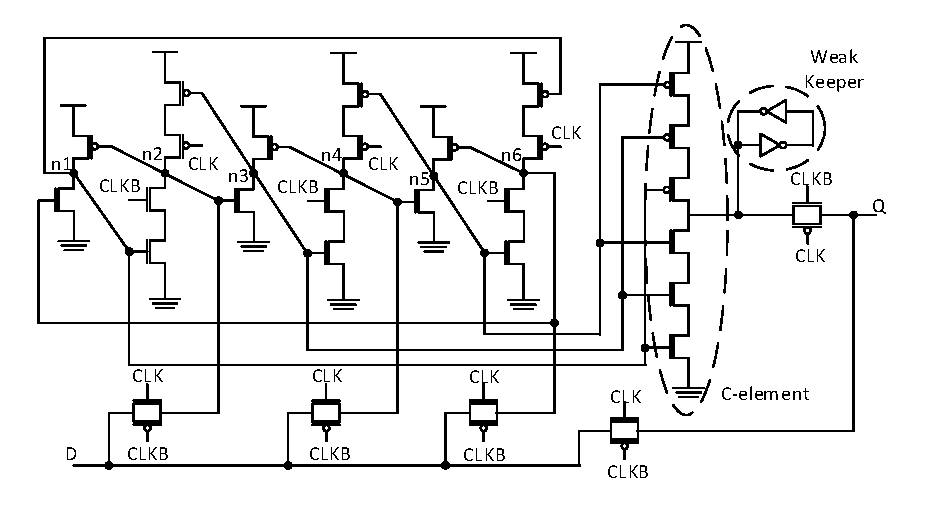
\includegraphics[width=\linewidth]{Figures/HSMUF}
	%where an .eps filename suffix will be assumed under latex, 
	%and a .pdf suffix will be assumed for pdflatex; or what has been declared
	%via \DeclareGraphicsExtensions.
	\caption{HSMUF latch \cite{HSMUF} with a weak keeper on the output.}
	\label{HSMUF_fig}
\end{figure}

To the author's knowledge, the most efficient existing DNU robust design is the DONUT latch \cite{DONUT} in Fig \ref{fig:DONUT}. The design, as proposed in their paper, uses only thirty-six transistors but has a much higher power consumption compared to the HSMUF (See Section \ref{sec:res}). The reason for high power consumption is due to contention on the input lines during the transparent mode. For example, if the node \textit{n2} in Fig. \ref{fig:DONUT} is observed during the transparent mode, the node is driven by three cross-coupled elements. This contention will increase the amount of time required to change the node thus drastically increasing the dynamic power consumption. To optimize their design, the 48 transistor DONUT-M latch was created in which each component connected to an input node is modified, as shown in Fig. \ref{DONUT_M}, so that the line is at high impedance for the whole duration of the transparent mode. This, in effect, removes the data contention problem thus reducing the overall dynamic power and delay.  

\begin{figure}[htbp]
	\centering
	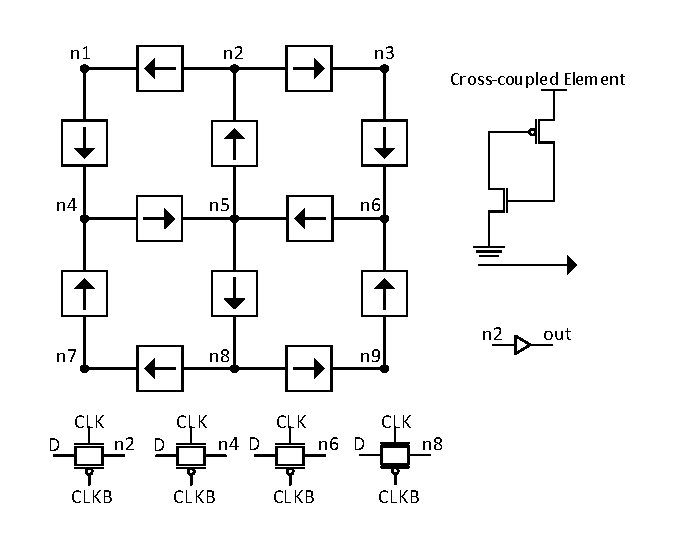
\includegraphics[width=0.65\linewidth]{Figures/DONUT}
	%where an .eps filename suffix will be assumed under latex, 
	%and a .pdf suffix will be assumed for pdflatex; or what has been declared
	%via \DeclareGraphicsExtensions.
	\caption{DONUT latch as proposed in \cite{DONUT}.}
	\label{fig:DONUT}
\end{figure}

\begin{figure}[htbp]
	\centering
	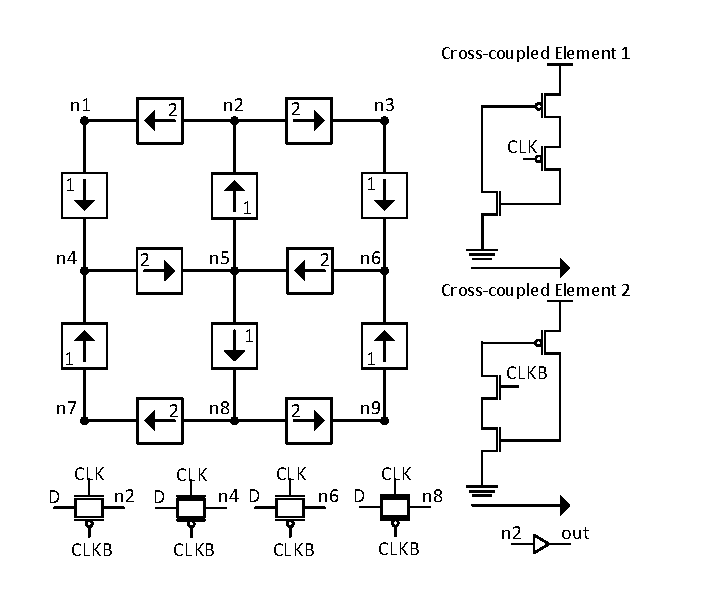
\includegraphics[width=0.65\linewidth]{Figures/ModDONUT}
	%where an .eps filename suffix will be assumed under latex, 
	%and a .pdf suffix will be assumed for pdflatex; or what has been declared
	%via \DeclareGraphicsExtensions.
	\caption{Modified low-power DONUT latch.}
	\label{DONUT_M}
\end{figure}

\section{Proposed HRDNUT Latch Design} \label{Proposed}
In this section the proposed DNU robust latch is discussed. The latch implementation is based on three cross connected storage loops connected to three C-elements. The basic design of the storage loop is given in Fig. \ref{Block}. The data loop is based on the standard latch design with a 3-input C-element inserted to replace one of the inverters. The purpose of the C-element is to separate the feedback loop so that an error will not be held. Additionally, a PMOS is connected to the positive clock signal (CLK) and a NMOS is connected to the negative clock signal (CLKB) to remove contention when data is loaded to the latch. As in the modified DONUT latch, the addition of these transistors drastically reduces the delay and power consumption.    

\begin{figure}[h]
	\centering
	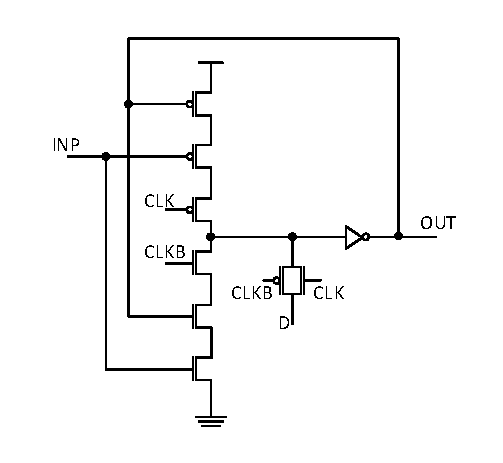
\includegraphics[width=0.5\linewidth]{Figures/Block}
	%where an .eps filename suffix will be assumed under latex, 
	%and a .pdf suffix will be assumed for pdflatex; or what has been declared
	%via \DeclareGraphicsExtensions.
	\caption{Basic data storage loop block.}
	\label{Block}
\end{figure} 

Using the basic storage block, the block based latch is constructed as in Fig. \ref{BLatch}. The latch was designed with the goal of ensuring that none of the nodes directly drove itself. For example, it can see that in Fig. \ref{Block} the node \textit{out} is fed into the input of the 3-input C-element. If an error strikes node \textit{out}, the cell will never be able to recover its previous state since one of the C-element inputs will be held to an erroneous value by its output. To prevent this issue, the design is based on cross-connecting three of the storage loop blocks so that the C-element is driven by three separate block outputs. In Fig. \ref{BLatch} a basic latch design using this idea is provided. If a single error occurs on any node in this design, the circuit is capable fully recovering the previous data. 

To demonstrate this, consider a strike on node \textit{n2}. When the strike occurs, the erroneous value will be propagated to the C-elements driving nodes \textit{n1} and \textit{n3}. However, since there is no change on \textit{n1} or \textit{n3}, the C-elements \textit{C1} and \textit{C3} will hold their previous value thus preventing the error from propagating to the output. Additionally, since node \textit{n2} is driven by nodes \textit{n1} and \textit{n3}, \textit{n2} will completely recover the correct state. 

\begin{figure}[!htbp]
	\centering
	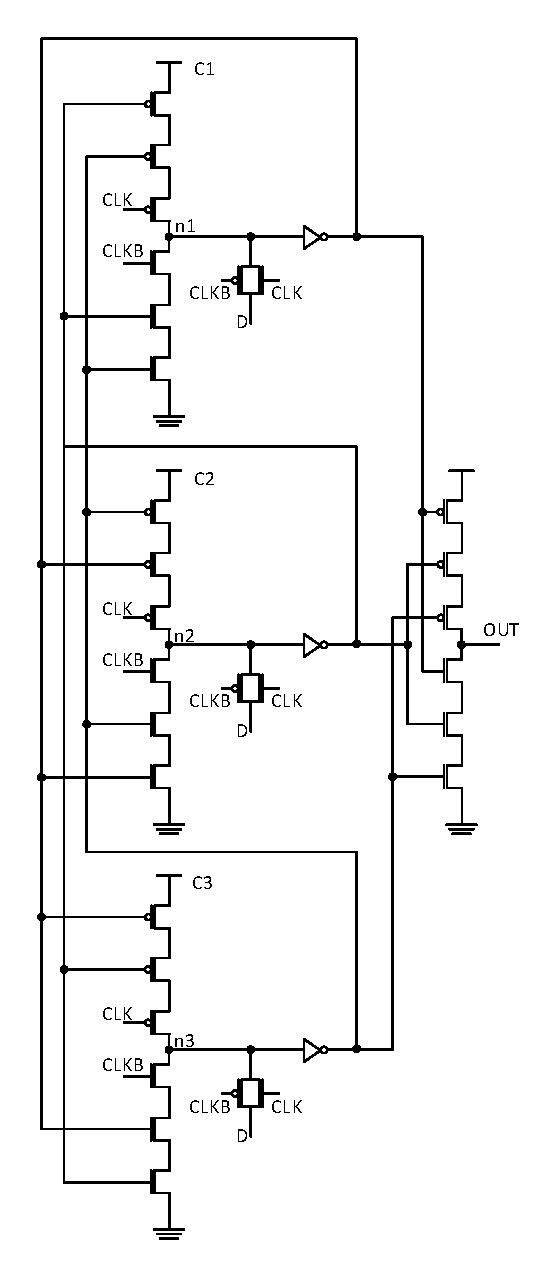
\includegraphics[width=0.55\linewidth]{Figures/BLatch}
	%where an .eps filename suffix will be assumed under latex, 
	%and a .pdf suffix will be assumed for pdflatex; or what has been declared
	%via \DeclareGraphicsExtensions.
	\caption{Schematic of the block-based latch.}
	\label{BLatch}
\end{figure} 

A problem, however, with the latch in Fig. \ref{BLatch} is that it is not capable of tolerating DNUs. For example, if an error occurs on nodes \textit{n1} and \textit{n2} the erroneous values will propagate to the inputs of C-element \textit{C3} and flip the value of \textit{n3} thus changing the output value. However, since the latch has recovery capability for SEUs, we modify it so it can tolerate DNUs and recover all nodes to the previous state. In Fig. \ref{HRDNUT} the schematic of the proposed HRDNUT latch is provided. The design uses the block-based latch in Fig. \ref{BLatch} as a base and adds additional C-elements to prevent errors from being held by the data loop.  

Initially, the HRDNUT latch is evaluated during normal operation. When the positive clock signal (CLK) has a high value and the negative clock signal (CLKB) has a low value, the latch is in transparent mode. At this stage, the transistors connected to the clock signal in C-element \textit{C1} deactivates the PMOS and NMOS stacks thus causing the node \textit{n1} to be in a high impedance state. This, in effect, reduces data contention thus reducing delay and dynamic power consumption. Next, the data is loaded through the pass gates connected to nodes \textit{n1}, \textit{n22} and \textit{out}. Since the output node \textit{out} is loaded directly, the propagation delay is minimized and all nodes are set to their respective error free values. When CLK changes to a low value and CLKB to a high value, the latch moves into the hold mode. In this stage, the pass gates are deactivated and the state of the latch is held since each node is driven to the correct value using a C-element. Fig. \ref{NormOp} provides the waveforms of the CLK, D and OUT nodes for both the transparent and hold modes of operation.

\begin{figure}[!htbp]
	\centering
	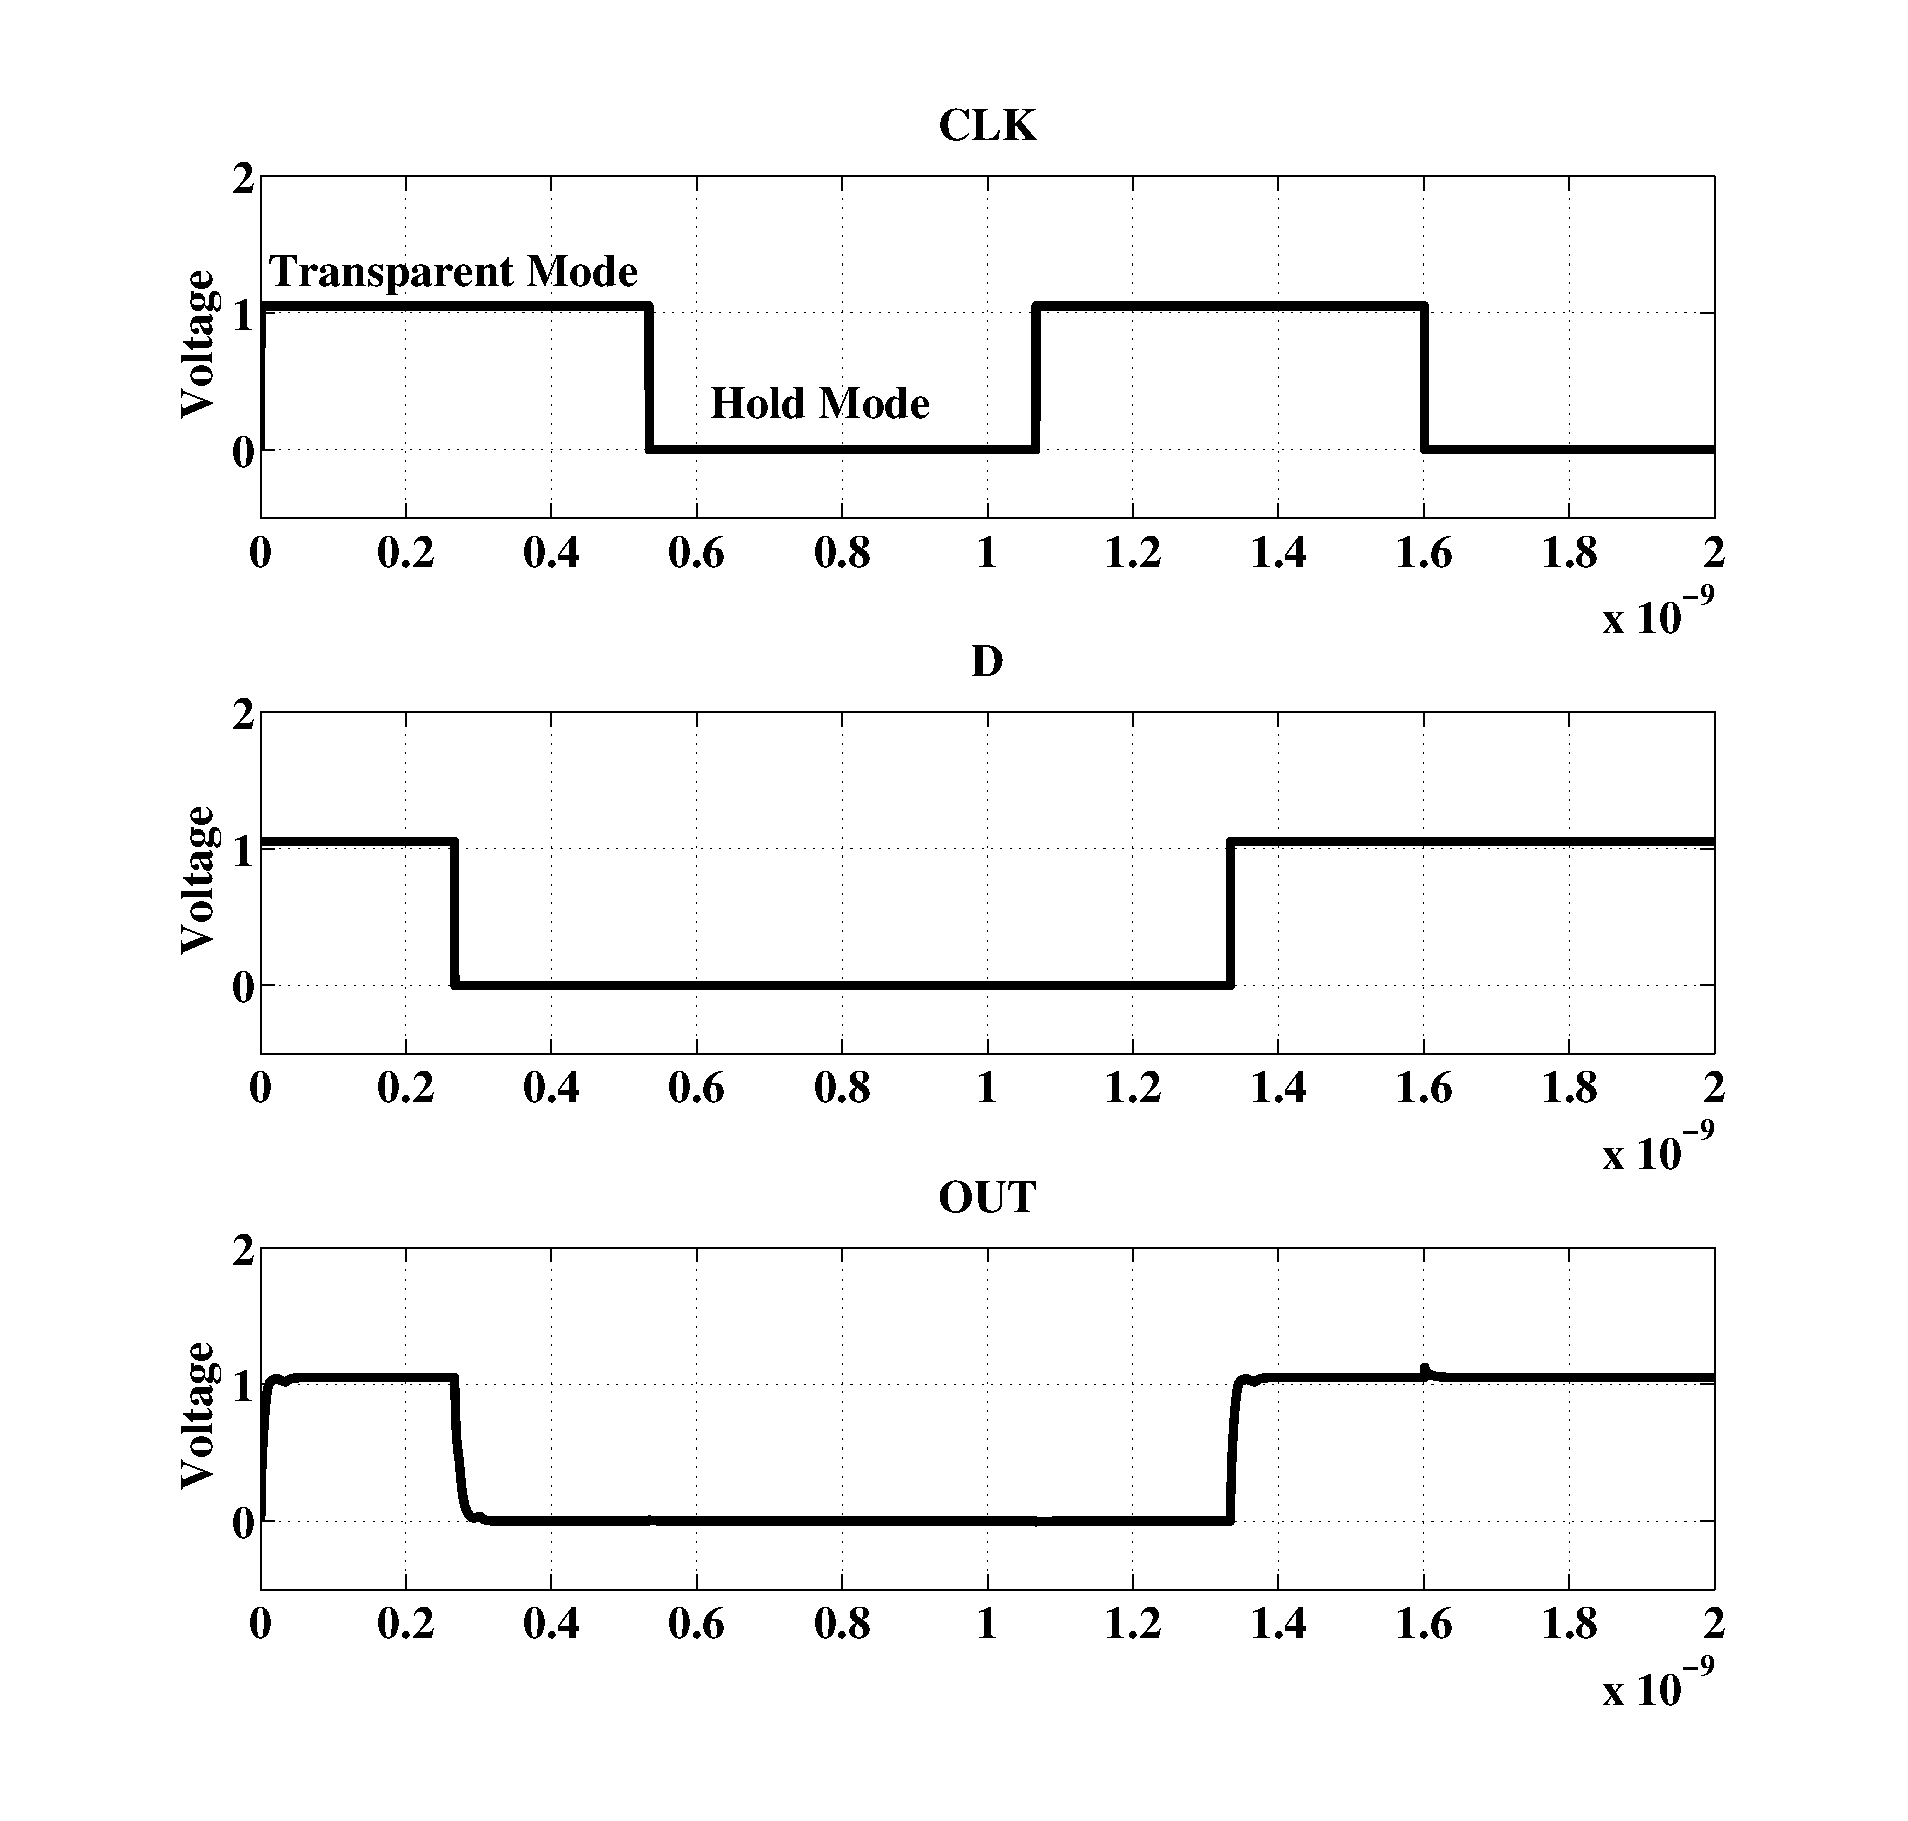
\includegraphics[width=0.65\linewidth]{Figures/defaultoperation.eps}
	%where an .eps filename suffix will be assumed under latex, 
	%and a .pdf suffix will be assumed for pdflatex; or what has been declared
	%via \DeclareGraphicsExtensions.
	\caption{Waveforms of the HRDNUT latch during normal operation.}
	\label{NormOp}
\end{figure}

In the case of an SEU, the HRDNUT retains the excellent resiliency of the block based latch and the ability to recover every node after an error. In the case of any internal node being struck by an error, the latch will not change value due to all internal C-elements requiring at least two identical input values to change the output. In the case of an error hitting the output node \textit{out}, the latch fully recovers since \textit{out} does not directly drive C-element \textit{C7}.

\begin{figure}[!tbp]
	\centering
	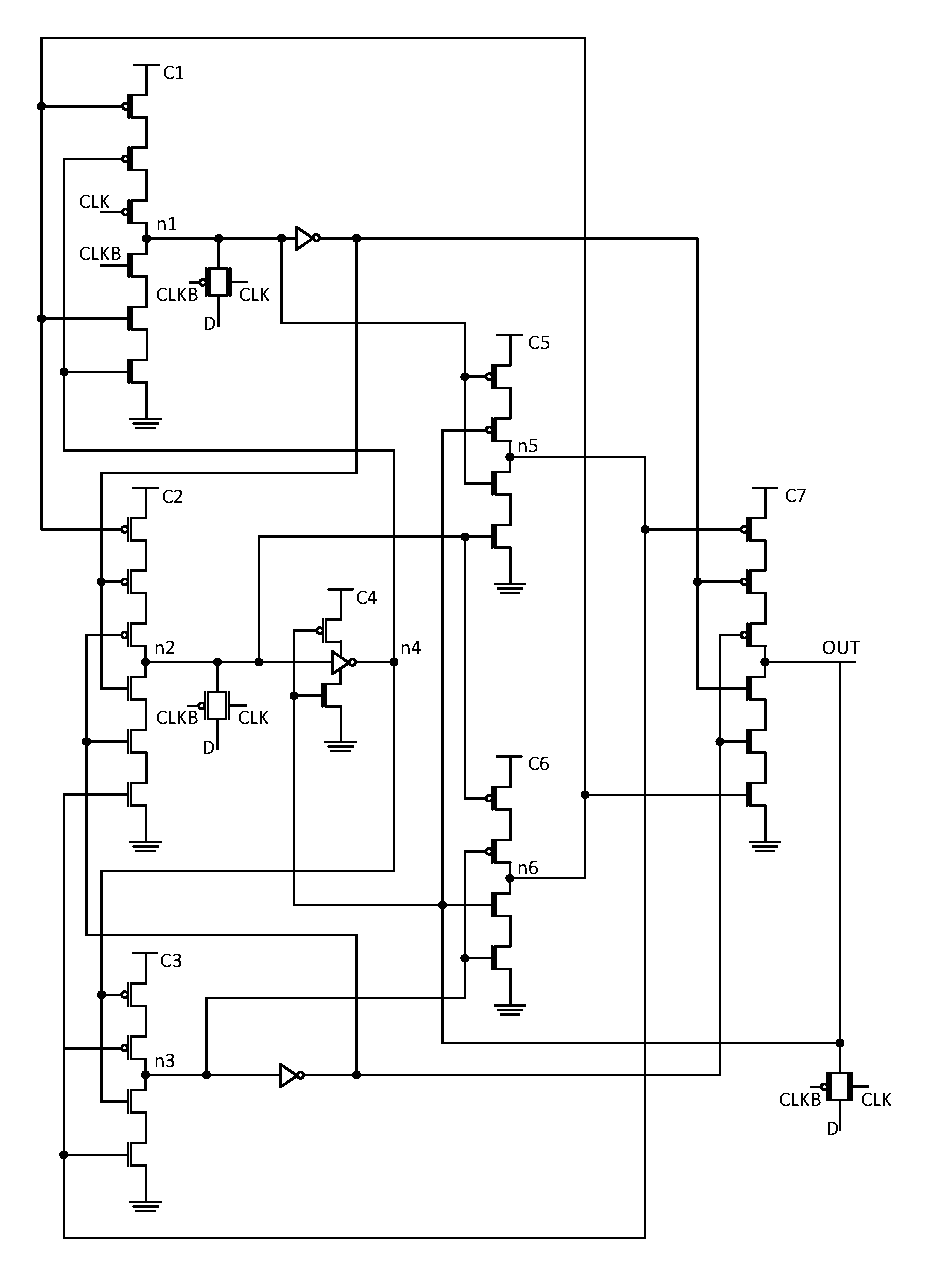
\includegraphics[width=0.95\linewidth]{Figures/HRDNUT}
	%where an .eps filename suffix will be assumed under latex, 
	%and a .pdf suffix will be assumed for pdflatex; or what has been declared
	%via \DeclareGraphicsExtensions.
	\caption{Schematic of the HRDNUT latch.}
	\label{HRDNUT}
\end{figure} 

Lastly, the latch will be evaluated in the case of a DNU. Note that unless otherwise stated, it is assumed that the analysis applies to both when D=0 and D=1. For the analysis, the possible DNU strike combinations are categorized into nine distinct cases based on their effect in the HRDNUT latch. Waveforms for each category can be found in Appendix \ref{Ap1}. The categories are discussed in detail below:

\begin{enumerate}
	\item Consider strikes at nodes \textit{n1} and \textit{n2}. In this case, the error at \textit{n1} will propagate to C-elements \textit{C5} and \textit{C7} but will not cause a flip since the error at \textit{n2} will be blocked by C-element \textit{C4}. Additionally, since the inputs of C-elements \textit{C1} and \textit{C2} are unchanged, the nodes will recover their initial values. This analysis can be applied to node combinations containing node \textit{n2} except for the combination with node \textit{out} since the error will be blocked by C-element \textit{C4}.
	
	\item In the case of a DNU upsetting nodes \textit{n2} and \textit{out}, the error at \textit{n2} will propagate through C-element \textit{C4}. However, C-elements \textit{C1} and \textit{C3} will block the error and nodes \textit{n1}, \textit{n3}, \textit{n5} and \textit{n6} will hold their values thus driving node \textit{out} to the correct state. 
	
	\item Consider when a DNU strikes nodes \textit{n1} and \textit{n5}. In this case, the error at \textit{n1} hits the output of C-element \textit{C1} which is propagated to \textit{C7}. The error on \textit{n5} is also propagated to C-element \textit{C7}. Since node \textit{n3} and the inputs of C-elements \textit{C1} and \textit{C5} are unaffected by an error, the output retains the error-free value and the latch fully recovers the previous state. The above analysis also applies to the node combination (\textit{n3}, \textit{n6}).
	
	\item In the case of a DNU hitting nodes \textit{n3} and \textit{n4}, the error at \textit{n4} is propagated to C-element \textit{C3} and the error at \textit{n3} is propagated to \textit{C7} and \textit{C6}. After the error on \textit{n3} subsides, \textit{C4} will drive node \textit{n4} and, due to the connection at \textit{C3}, node \textit{n3} back to the error-free value. The node combination (\textit{n1}, \textit{n1}) can be analyzed similarly. For the node combinations of (\textit{n4}, \textit{n5}) and (\textit{n4}, \textit{n6}), the latch will also recover the previous result since the inputs to \textit{C4} are unchanged. This implies that after the error occurs at \textit{n4}, the node will be driven back to the correct value thus also driving the nodes \textit{n5} or \textit{n6} back to the correct value.
	
	\item When a DNU upsets the combination of \textit{n4} and \textit{out}, the error at \textit{out} is propagated to \textit{C4}, \textit{C5} and \textit{C6} and the error at \textit{n4} to \textit{C1} and \textit{C3}. Since none of the inputs to \textit{C7} are changed by the error, \textit{out} is reverted back to its error-free value which drives \textit{n4} through \textit{C4} back to its previous state.
	
	\item Consider when a DNU strikes nodes \textit{n1} and \textit{n3} being struck. In this case, the errors are propagated to C-elements \textit{C2}, \textit{C5}, \textit{C6} and \textit{C7}. However, because the errors do not manifest into an error on any other node, the latch fully recovers from the error. 
	
	\item When a DNU strikes the nodes \textit{n1} and \textit{n6}. The error at node \textit{n6} propagates to  \textit{C1} and \textit{C7} while the error at \textit{n1} also propagates to \textit{C7}. Due to the error-free node \textit{n3} driving \textit{C7}, the previous value is held at the output by \textit{C7}. Additionally, \textit{n3} will drive \textit{C6} back to its previous value thus driving \textit{C1} back to the error free state. This analysis can be applied similarly to the node combination of (\textit{n3}, \textit{n5}). 
	
	\item In the case where a DNU strikes nodes \textit{n5} and \textit{out} the error at \textit{n5} propagates to \textit{C7}, \textit{C2} and \textit{C3} and the error at \textit{out} goes to \textit{C4}, a PMOS in \textit{C5} and a NMOS in \textit{C6}. When the error-free value at \textit{out} is 1, the value at \textit{n5} is 0. The error at the nodes change the values to 0 and 1 respectively and the erroneous value at \textit{out} is propagated to the PMOS at \textit{C5} and the NMOS at \textit{C6}. This, in effect, causes the PMOS at \textit{C5} to be activated and the NMOS at \textit{C6} to be deactivated. However, since nodes \textit{n1} and \textit{n2} remain error-free, the NMOS stack of \textit{C5} will drive \textit{n5} back to the correct value. This, in turn, forces \textit{C7} to also drive \textit{out} back to the error-free value. In the case where \textit{out} has an ideal value of 0, the error will be fully recovered since the NMOS stack will be entirely driven by fault-free nodes. The above analysis can be applied to the node combination of (\textit{n6}, \textit{out}). 
	
	\item Lastly, the node combinations (\textit{n1}, \textit{out}), (\textit{n3}, \textit{out}) and (\textit{n5}, \textit{n6}) are analyzed. In these cases the errors do not cause a change on the inputs of any C-elements driving the node thus the previous value will always be recovered. 
\end{enumerate}

\section{Simulation Results} \label{sec:res}
The proposed HRDNUT latch has been implement using the 1.05V 32 nm PTM library \cite{PTM} and simulated in HSPICE. All transistors were set to the minimum size with the PMOS widths set to W=80 nm and the NMOS widths set to W=40 nm. To evaluate the DNU reliability of the design, current pulses were injected for every possible error combination. The injection current was calculated using the equation found in \cite{injeq}. The equation is given below with $\tau$ as the technology dependent constant, $Q_o$ as the injection current value and $t$ as the variable for time. 

\begin{equation}\label{qeq}
I(t)=\frac{2Q_o}{\tau\sqrt{\pi}}\sqrt{\frac{t}{\tau}}e^{\frac{-t}{\tau}}
\end{equation}

Using equation (\ref{qeq}) $\tau$ was set to $32\times10^{-12}$ and $Q_o$ was set to $5\text{fC}$. In all simulations, the latch was operated at a frequency of 1Ghz. In Appendix I Figs. \ref{fig:CLK}-\ref{fig:n5n6}, the waveforms for each case discussed in Section \ref{Proposed} are presented and show that the HRDNUT is fully capable of recovering all nodes in the presence of a DNU. 

Next, the HRDNUT is compared to existing SEU and DNU tolerant methods. As in the HRDNUT latch, all latches were designed using the 32nm PTM library and operated at 1Ghz. For the analysis, the following SEU tolerant latches were compared: DICE \cite{DICE}, FERST \cite{FERST} and HIPER \cite{HIPER}. Additionally, the following DNU tolerant designs are also analyzed: DNCS \cite{DNCS}, Interception \cite{Inter}, HSMUF \cite{HSMUF} and DONUT \cite{DONUT}. All transistors for the implemented latches were set to minimum width and length except for the designs that use a C-element with a weak keeper. In these designs the C-element's PMOS width was set to W=320 nm and the NMOS width was set to W=160 nm. The weak keeper was sized to be at minimum width. The C-element was sized so that the output driving strength did not allow the keeper to drive an erroneous value in the event of an error. 

To provide a fair comparison, the propagation delay, average power consumption and area of all designs is measured and each design is categorized based on whether they can tolerate a DNU and if they are DNU robust. The delay was measured as the time between when a transition occurs on input \textit{D} to when a transition was observed on the output. The average power was computed using the error-free operation for each latch for a duration of 200 ns. To compare the area overhead, the unit size transistor (UST) metric was adopted as in \cite{DNCS} which represents the number of unit sized (minimum width is W=40 nm in this case) transistors required for the design. Table \ref{table:rtable} provides the results of these simulations.

\begin{table}[h]
	\begin{center}
		\caption{SPICE Simulations of Existing Latches using the 1.05V 32nm PTM library }
		\label{table:rtable}
		\begin{tabular}{|m{8em}|m{5em}|m{5em}|m{3em}|m{3em}|m{3em}|}
			\hline
			Latch & DNU Immune & DNU Robust & Power ($\mu$W) & Delay (ps) & Area (UST)\\ 
			\hline
			DICE & No & No & 1.332 & 8.145 & 16 \\
			\hline
			FERST & No & No & 3.178 & 31.648 & 60 \\
			\hline
			HIPER & No & No & 1.292 & 2.221 & 27 \\
			\hhline{|=|=|=|=|=|=|}
			DNCS & Yes & No & 4.948 & 22.486 & 61 \\
			\hline
			\cite{Inter} & Yes & No & 5.606 & 79.168 & 89 \\
			\hline
			HSMUF & Yes & No & 1.871 & 1.0626 & 51 \\
			\hline
			HSMUF (Keeper) & Yes & No & 3.787 & 3.945 & 78 \\
			\hhline{|=|=|=|=|=|=|}
			DONUT \cite{DONUT} & Yes & Yes & 4.021 & 14.722 & 54 \\ 
			\hline
			DONUT-M \newline (Section \ref{sec:DNUex}) & Yes & Yes & 2.760 & 8.421 & 72\\
			\hline
			HRDNUT \newline (Proposed) & Yes & Yes & 2.450 & 2.310 & 66 \\
			\hline
		\end{tabular}
	\end{center}
\end{table}

According to Table \ref{table:rtable} the only DNU robust designs are the two DONUT latch implementations and the HRDNUT. Compared to the modified DONUT latch, the HRDNUT provides DNU robustness while reducing the power consumption and the number of transistors by 11.3\% and 8.33\% respectively while also reducing the delay by 72.5\%. For the above reasons, the HRDNUT is the best design for clock gating applications due to its robustness and lower power, delay and area overheads.

\section{Filtering of Transients Arriving on the Latch Input}
In addition to radiation particles hitting the internal nodes in a latch, transient voltage pulses may arrive on the inputs of a combinational circuit. In a typical digital system design, combinational logic is placed between two sets of flip-flops, one set driving the input and the other being driven by the output of the combinational circuit. While there are masking factors in combinational circuits, they may still allow a pulse to arrive on the input of a flip flop. A novel circuit to filter incoming pulses was proposed in \cite{FERST} and is given in \ref{P_filter}. Their design consisted of routing the pulse through two paths, one with no delay and one with sufficient delay that the two pulses will not overlap. The general design is given below.

\begin{figure}[!htbp]
	\centering
	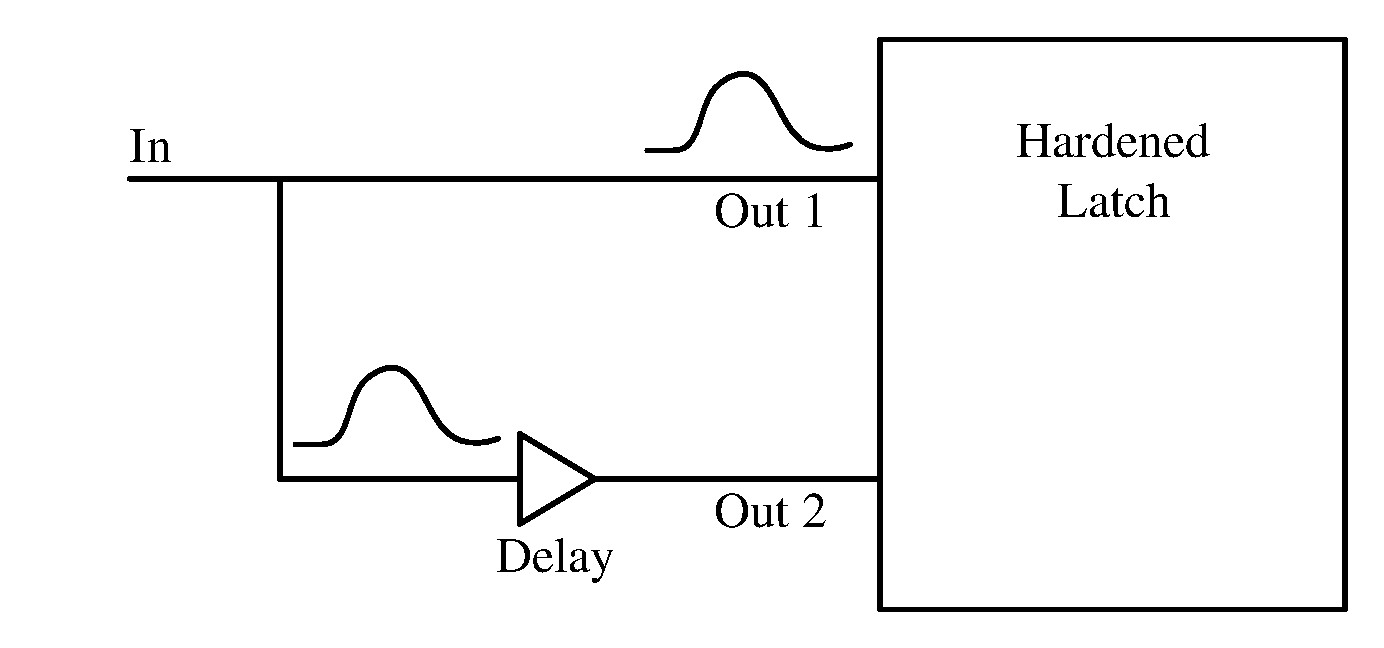
\includegraphics[width=0.65\linewidth]{Figures/PulseFilter}
	%where an .eps filename suffix will be assumed under latex, 
	%and a .pdf suffix will be assumed for pdflatex; or what has been declared
	%via \DeclareGraphicsExtensions.
	\caption{The pulse filtering circuit provided in \cite{FERST}.}
	\label{P_filter}
\end{figure}

An issue with the approach in Fig. \ref{P_filter} is that in a radioactive environment, a high energy particle can hit the delay element causing a voltage pulse on the node. If this occurs while a pulse is being propagated through the circuit, it could create a secondary pulse at the delay element causing an erroneous value to be latched in the flip flop. A simple way to mitigate this effect is to add an additional delay element with twice the delay. This, in effect, will allow the device to function properly even if an error occurs during the filtering stage. The design of the device is given in Fig. \ref{Enh_filter}. Due to the use of three outputs, the device can be used with the HRDNUT latch without modification.

\begin{figure}[!htbp]
	\centering
	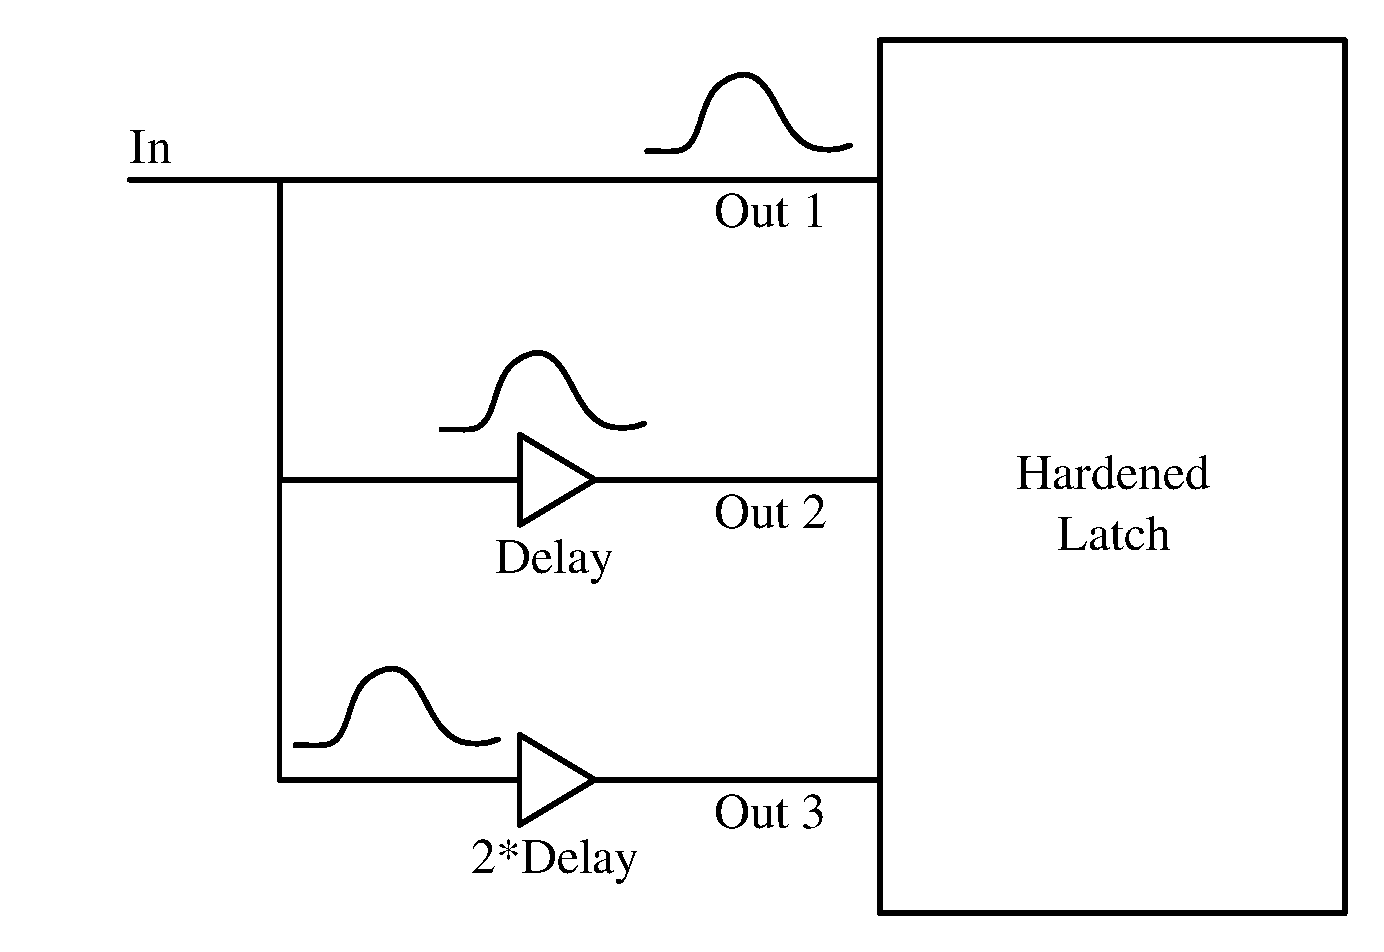
\includegraphics[width=0.65\linewidth]{Figures/PulseFilterEnh}
	%where an .eps filename suffix will be assumed under latex, 
	%and a .pdf suffix will be assumed for pdflatex; or what has been declared
	%via \DeclareGraphicsExtensions.
	\caption{The enhanced pulse filtering circuit that can tolerate an error.}
	\label{Enh_filter}
\end{figure} 

Next the filtering circuit is evaluated. If a pulse arrives on node $In$, it is propagated to the three delay elements. The pulse arriving on $OUT1$ will propagate to the latch with no increased delay. The pulse on $OUT2$ will arrive at the latch with a delay of one unit and the pulse on $OUT3$ will arrive with a delay of two units. If an error occurs on the buffer at $OUT3$ while a pulse is being propagated, an additional pulse will be generated at the buffer causing two node to simultaneously have the same data value. However, since node $OUT2$ is error free during this stage, the circuit will still filter the pulse allowing the correct data to be latched. This analysis can be applied similarly to the case where a strike occurs on the buffer connected to $OUT2$.

To determine the power overhead of the filtering circuit, the device was implemented in the 32 nm PTM library and operated at 1 Ghz. The circuit was designed to filter pulses with a width of 20 ps. This was accomplished using a chain of four buffers for the short delay and eight buffers for the long delay which had a 5 ps propagation delay each. Simulations were completed in HSPICE which show that the addition of the filtering circuit increases the power consumption by 3.15 ps and has a minimum delay of 40 ps.

\section{Towards the Design of a Triple Node Upset Tolerant Latch}
An inevitable issue with the development of more complex latches to tolerate multiple errors is the increase of the number of transistors and area. This issue leads to the possibility of new latch designs being vulnerable to more simultaneous error such as a triple node upset (TNU). The goal of this section is to estimate the area and device overhead and to evaluate the feasibility of a TNU tolerant latch. To begin the analysis, the design methodology used in the development of the HRDNUT is applied. The basic element used in this design is the block based latch given in Fig. \ref{BLatch}. In the case of the HRDNUT, 3 blocks were needed to harden the latch against 2 errors. Based on this observance, it is estimated that hardening against TNUs will require 4 blocks. Additionally, to hold to the principle discussed earlier in this paper that no element drives itself, each c-element will have an additional transistor added to accompany the extra block. The block based latch for TNUs is given in Fig. \ref{TNUB} which has 56 total transistors. Since the block based latch for the HRDNUT has 36 transistors, it can be extrapolated that TNU hardening requires a 35\% transistor overhead.

\begin{figure}[!htbp]
	\centering
	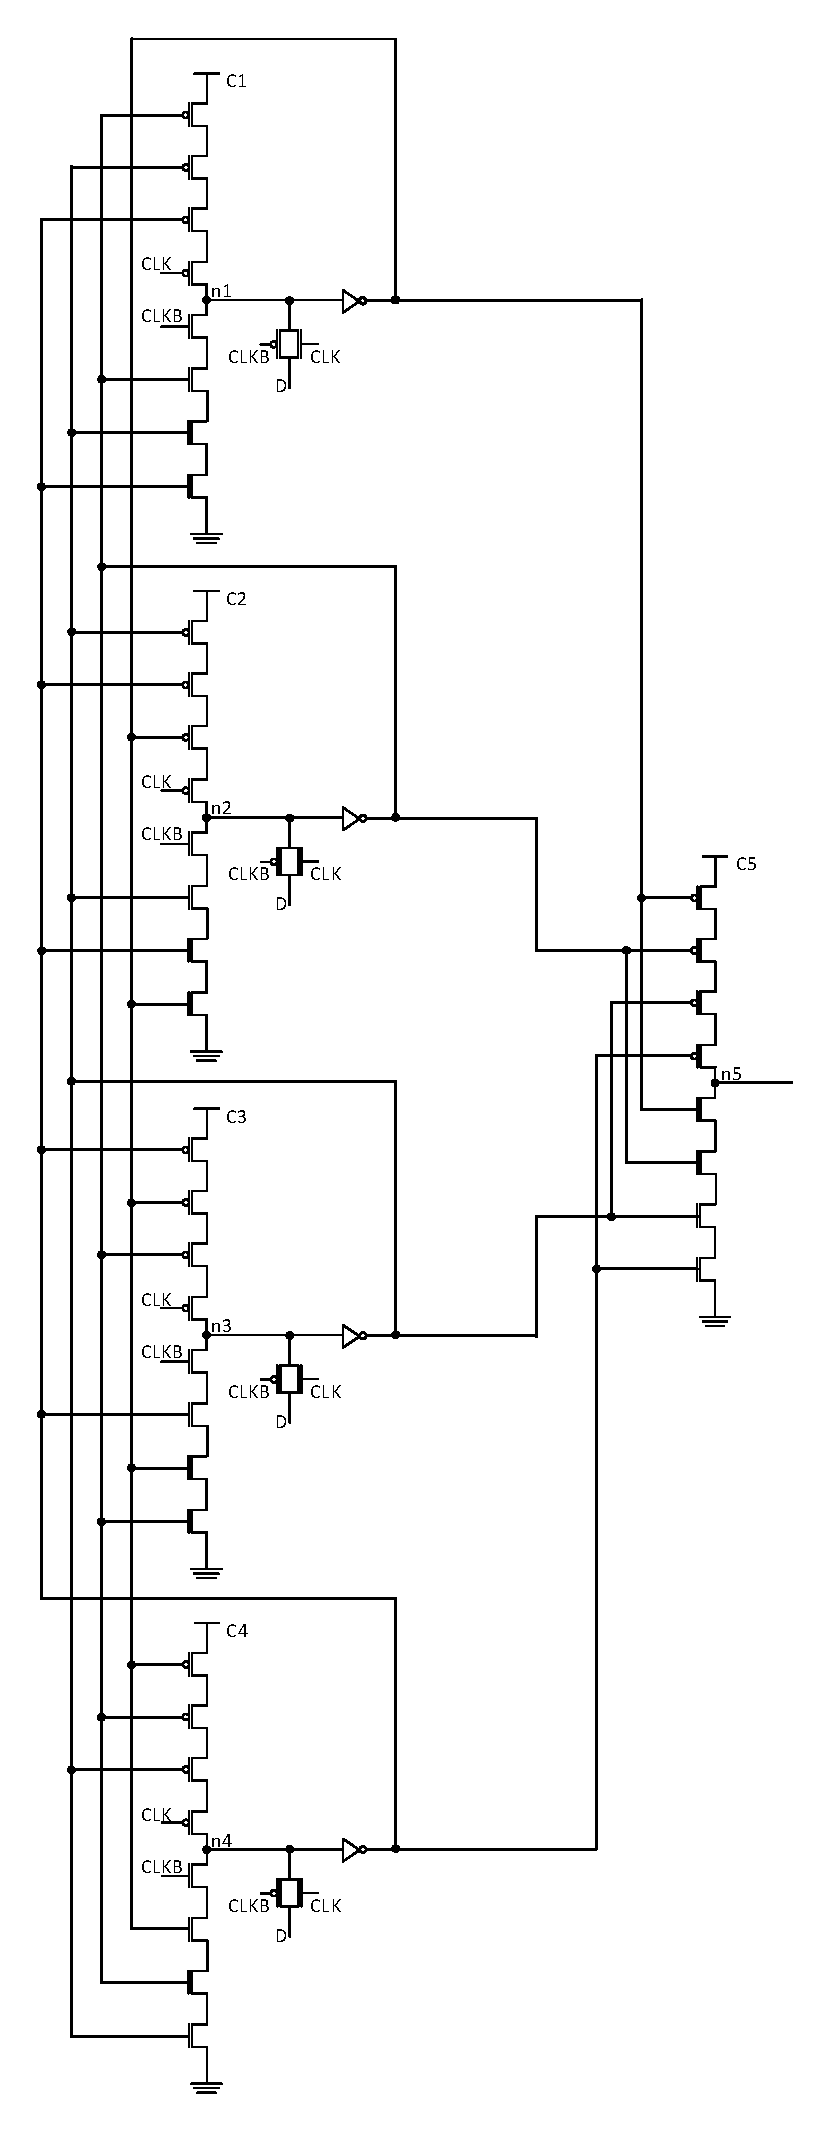
\includegraphics[width=0.50\linewidth]{Figures/TNUBlatch}
	%where an .eps filename suffix will be assumed under latex, 
	%and a .pdf suffix will be assumed for pdflatex; or what has been declared
	%via \DeclareGraphicsExtensions.
	\caption{Block based latch that forms the basis for a TNU tolerant design.}
	\label{TNUB}
\end{figure}

To further estimate the power, delay and area overheads of a TNU latch, a design, provided in Fig. \ref{TNULatch}, was created which shows promise of being TNU tolerant and robust. It is based on the ideas used for the HRDNUT and derived from the TNU block latch. Due to it being based on the HRDNUT, it can be assured that it is both SEU and DNU tolerant. For each cases tested, the latch has been shown to be TNU tolerant. However, to fully verify TNU tolerance, the design must be tested for 165 total TNU cases. For the sake of discussion, three examples of how the latch tolerates a TNU are given below.  

\begin{enumerate}
	\item Consider a TNU on nodes \textit{out}, \textit{n5} and \textit{n6}. The error at \textit{n5} will effect C-elements \textit{C1, C3, C4} and \textit{C9}. The transient at \textit{n6} will effect nodes \textit{C1, C2, C4} and \textit{C8}. Lastly, the error at \textit{out} will arrive at C-elements \textit{C5} and \textit{C6}. In this case, the output node will directly be driven back to the correct value due to no change on any of the inputs on C-element \textit{C11}. Since \textit{out} is driven back to the correct value, all of the inputs on C-elements \textit{C5} and \textit{C6} are returned back to the error free value. This will, in turn, drive nodes \textit{n5} and \textit{n6} back to the correct value thus fully recovering all nodes.
	
	\item Assume a TNU strikes nodes \textit{n7, n8} and \textit{out}. Node \textit{n7} has a transient that propagates to C-element \textit{C11}. Similarly, node \textit{n8} also has a transient propagates to \textit{C11}. The transient pulse on node \textit{out} arrives on the inputs of C-elements \textit{C5} and \textit{C6}. In this case, all transient pulses are blocked by the respective C-element since not each element has at least one error-free input. This implies that all nodes will fully recover to their respective value.
	
	\item Consider a TNU that generates pulses on nodes \textit{n9, n2} and \textit{out}. In this case, the errors on the nodes will flip the output of C-element \textit{C5} thus also causing a transient on node \textit{n5}. The error on \textit{n5} will propagate to C-elements \textit{C1, C3, C4} and \textit{C10}. However, the pulse will be blocked at all elements. Additionally, since \textit{n2, n9} and \textit{out} all restored to their error free value, \textit{n5} will also return to the correct value.
\end{enumerate}

\begin{figure}[!htbp]
	\centering
	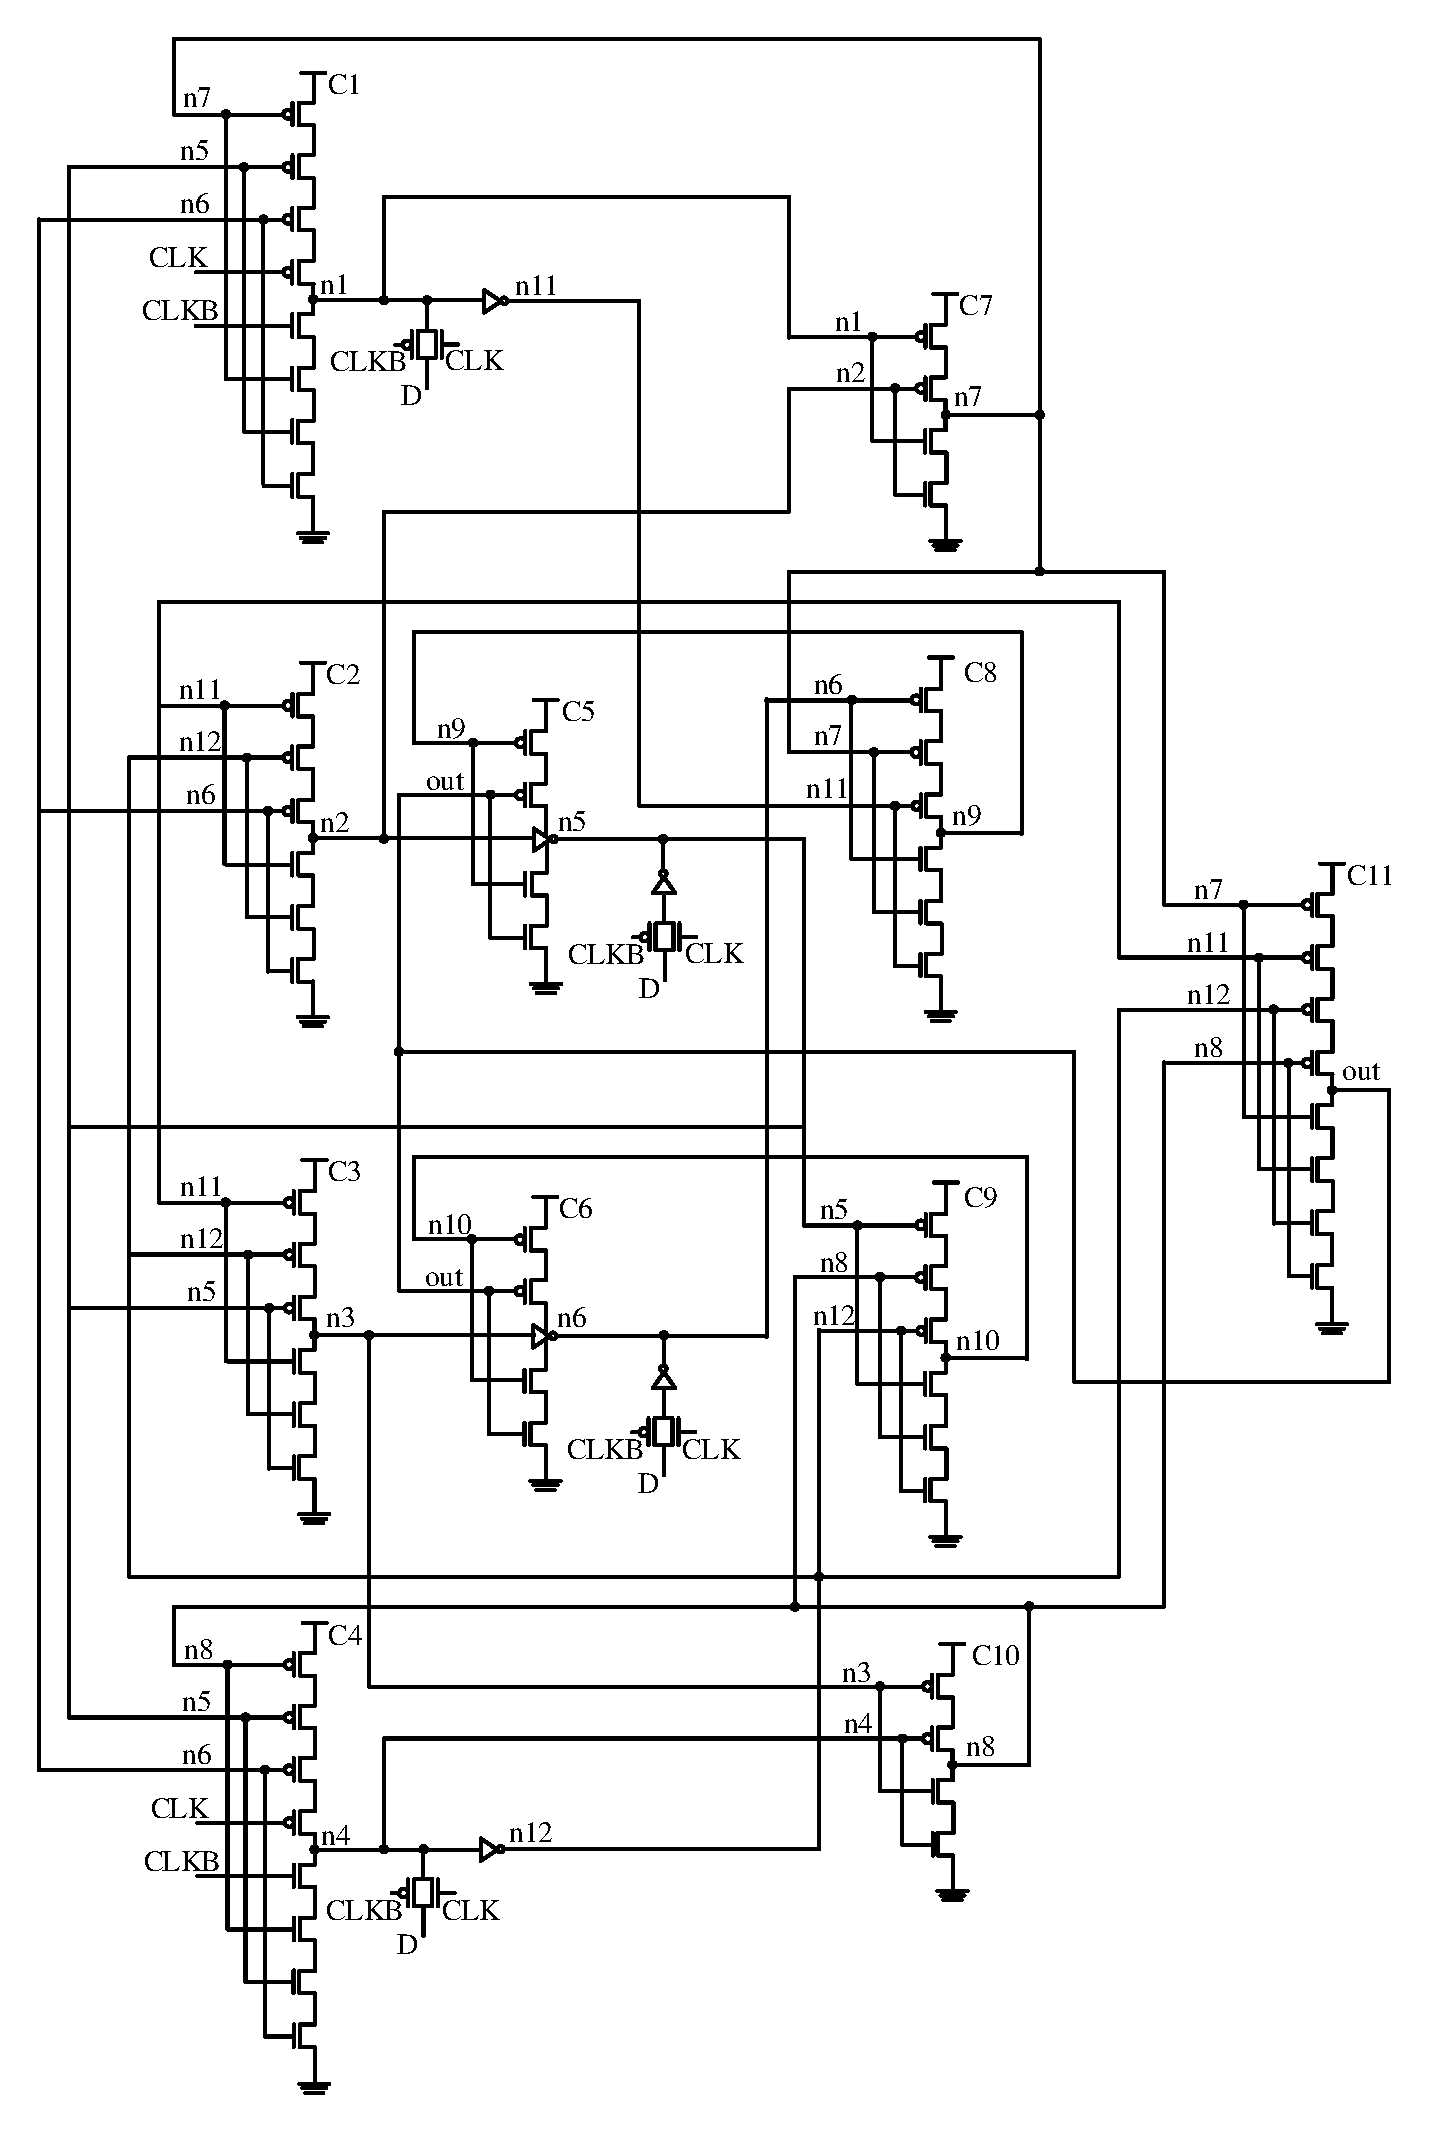
\includegraphics[width=0.90\linewidth]{Figures/TNULatch2}
	%where an .eps filename suffix will be assumed under latex, 
	%and a .pdf suffix will be assumed for pdflatex; or what has been declared
	%via \DeclareGraphicsExtensions.
	\caption{Schematic of the TNU tolerant latch.}
	\label{TNULatch}
\end{figure} 

The design was implemented in HSPICE using the 32nm PTM library with all transistors set to minimum width (PMOS=80nm, NMOS=40nm). The clock frequency was set to 1Ghz and $V_{dd}$ to 1.05V. The latch was operated with no injected transient pulses to measure the average power. It was found that the TNU latch consumes 4.09 $\mu$W which is 60\% higher compared to the HRDNUT. Furthermore, the TNU tolerant design has an UST area of 129 and delay of 2.77 ps, which is double that of the HRDNUT. 

Based on the design, there are few similarities to the HRDNUT that have been observed that can be used to design latches that tolerate four or more errors. The similarities are summed up in the following list:

\begin{enumerate}
	\item Assuming the latch will tolerate a $n$ number of errors, the block based latch will have $n+1$ number of elements.
	\item Each storage block in the block based latch will have at least one C-element with a $n$ number of inputs.
	\item At least one of the blocks will have two C-elements with a $n$ number of inputs.
	\item Each block should be wired such that no wire drives itself. This is to ensure robustness.
	\item An intermediary level of C-elements must be inserted between the blocks and the output device to ensure robustness.
	\item The output must be looped back to drive a C-element.
	\item To load data to the latch, a $n+1$ number of nodes must be driven by the data line. 
	\item At least one C-element will be set to high impedance during the transparent mode to increase performance.
\end{enumerate}
 
\section{Conclusion} \label{sec:conc}
In this section the HRDNUT latch was proposed which is suited for clock gating schemes. Since clock gating may require the latch to remain in a hold state for many clock cycles, the susceptibility of error increases. In many existing designs, a DNU may either change the state of the latch or push the latch into a state were the output may discharge over time due to a high impedance state. A common method to solve this problem is the addition of a weak keeper on the output. As shown in this paper, the addition of the keeper causes much higher power consumption. Since the HRDNUT latch does not stay in a high impedance state after a DNU, the HRDNUT provides high reliability during the whole duration of the hold mode while providing the lowest delay, power and area compared to other latches suitable for clock gating. Simulation results show that the HRDNUT is 11.3\% more power efficient while requiring 8\% less transistors and 72.5\% less delay compared to the highly robust DONUT latch. 

Additionally, an enhanced circuit to filter incoming transient pulses was proposed. The new circuit is able to tolerate a single error during the filtering phase. The area additional area of the new filter circuit is dependent on the size of the expected transient but overall is low. Lastly, an analysis of the TNU was conducted and the block based circuit was given. It was determined that a TNU tolerant circuit would have a 35\% greater overhead compared to the HRDNUT. Based off this finding, it is recommended that a TNU tolerant latch is used in extreme radiation environments where system stability is crucial.